\chapter[Encoder-Only Transformers: BERT and JEPA]{Encoder-Only Transformers: BERT, Representations, and JEPA}
\label{ch:bert}

\section{The Rise and Repositioning of BERT}

In 2019, BERT held the top score on many major NLP benchmarks---reading comprehension, sentiment analysis, textual entailment, question answering. A single pretrained model, fine-tuned with a small task-specific head, outperformed years of carefully engineered pipelines. The recipe was simple: pretrain a deep bidirectional Transformer on raw text, then fine-tune on labeled data. NLP had its ImageNet moment.

By 2023, frontier general-purpose AI efforts were no longer scaling BERT-style encoders as the main route to capability. The architecture didn't get worse. The world changed around it.

This chapter tells that story---not as a cautionary tale, but as a lens for understanding what different Transformer architectures are actually good at. Chapter~\ref{ch:decoder-only} showed how a decoder-only Transformer generates text by predicting the next token. This chapter shows how the \emph{same} Transformer block, with two changes---remove the causal mask, replace next-token prediction with masked language modeling---becomes something fundamentally different: a machine for learning bidirectional representations.

\begin{quickrecap}
\textbf{The core contrast.}
\begin{itemize}[nosep,leftmargin=1.5em]
  \item \textbf{GPT (Ch3):} causal mask + next-token prediction $\to$ generation.
  \item \textbf{BERT (this chapter):} bidirectional attention + masked language modeling $\to$ representation.
  \item Same mechanism, different objective, different capability.
\end{itemize}
\textit{Historically, BERT (2018) appeared before GPT-2 (2019). We present it second because its design is best understood as a deliberate departure from causal language modeling---and because decoder-only models are the backbone of modern LLMs.}
\end{quickrecap}


\subsection*{Learning Objectives}

After completing this chapter, you should be able to:

\begin{enumerate}
  \item Explain why removing the causal mask enables bidirectional context and why this helps representation tasks but prevents autoregressive generation.
  \item Describe masked language modeling (MLM): what gets masked, what gets predicted, and why the 80/10/10 strategy exists.
  \item Trace BERT's input format: \texttt{[CLS]}, \texttt{[SEP]}, segment embeddings, and how task-specific heads attach to the pretrained body.
  \item Articulate why BERT lost the frontier role: training signal sparsity, inability to generate, and fine-tuning fragility.
  \item Compare BERT's input-space masked prediction with JEPA's latent-space prediction, and explain why the latter may be more sample-efficient for representation learning.
\end{enumerate}

\subsection*{Notation}

\begin{center}
\begin{tabular}{ll}
\toprule
Symbol & Meaning \\
\midrule
$T$ & Sequence length \\
$d_{\text{model}}$ & Hidden dimension \\
$V$ & Vocabulary size \\
$p_{\text{mask}}$ & Masking probability (typically 0.15) \\
$\texttt{[CLS]}$ & Special classification token (position 0) \\
$\texttt{[MASK]}$ & Placeholder token replacing masked positions \\
\bottomrule
\end{tabular}
\end{center}

\subsection*{Timeline}

\begin{center}
\begin{tabularx}{\textwidth}{@{}lp{3.5cm}X@{}}
\toprule
Year & Contribution & Key idea \\
\midrule
2018 & ELMo~\cite{peters2018elmo} & Contextual embeddings from bidirectional LSTMs \\
2018 & GPT-1~\cite{radford2018improving} & Unidirectional Transformer pretraining + fine-tuning \\
2018 & BERT~\cite{devlin2019bert} & Bidirectional Transformer with MLM; pre-train + fine-tune at scale \\
2019 & RoBERTa~\cite{liu2019roberta} & Remove NSP, train longer on more data, dynamic masking \\
2019 & Sentence-BERT~\cite{reimers2019sentence} & Siamese BERT for sentence embeddings \\
2020 & DeBERTa~\cite{he2020deberta} & Disentangled attention: separate content and position \\
2022 & JEPA concept~\cite{lecun2022path} & Predict in latent space, not input space \\
2023--25 & I-JEPA / V-JEPA~\cite{assran2023ijepa,bardes2024vjepa,vjepa2meta2025} & JEPA validated on images and video \\
2024--25 & BGE, E5, GTE & Modern encoder-only embedding models \\
\bottomrule
\end{tabularx}
\end{center}


%----------------------------------------------------------------------
\section{Encoder-Only Attention: Removing the Causal Mask}
\label{sec:bidirectional}

Recall from Chapter~\ref{ch:decoder-only} that a decoder-only Transformer masks out all future positions: token $t$ can only attend to tokens $1, \ldots, t$. This is necessary for autoregressive generation---the model must not ``see the answer'' during training.

But what if we don't need to generate? What if the goal is not to produce text token by token, but to \emph{understand} a complete input---classify its sentiment, extract named entities, answer a question about it?

\begin{figure}[ht]
\centering
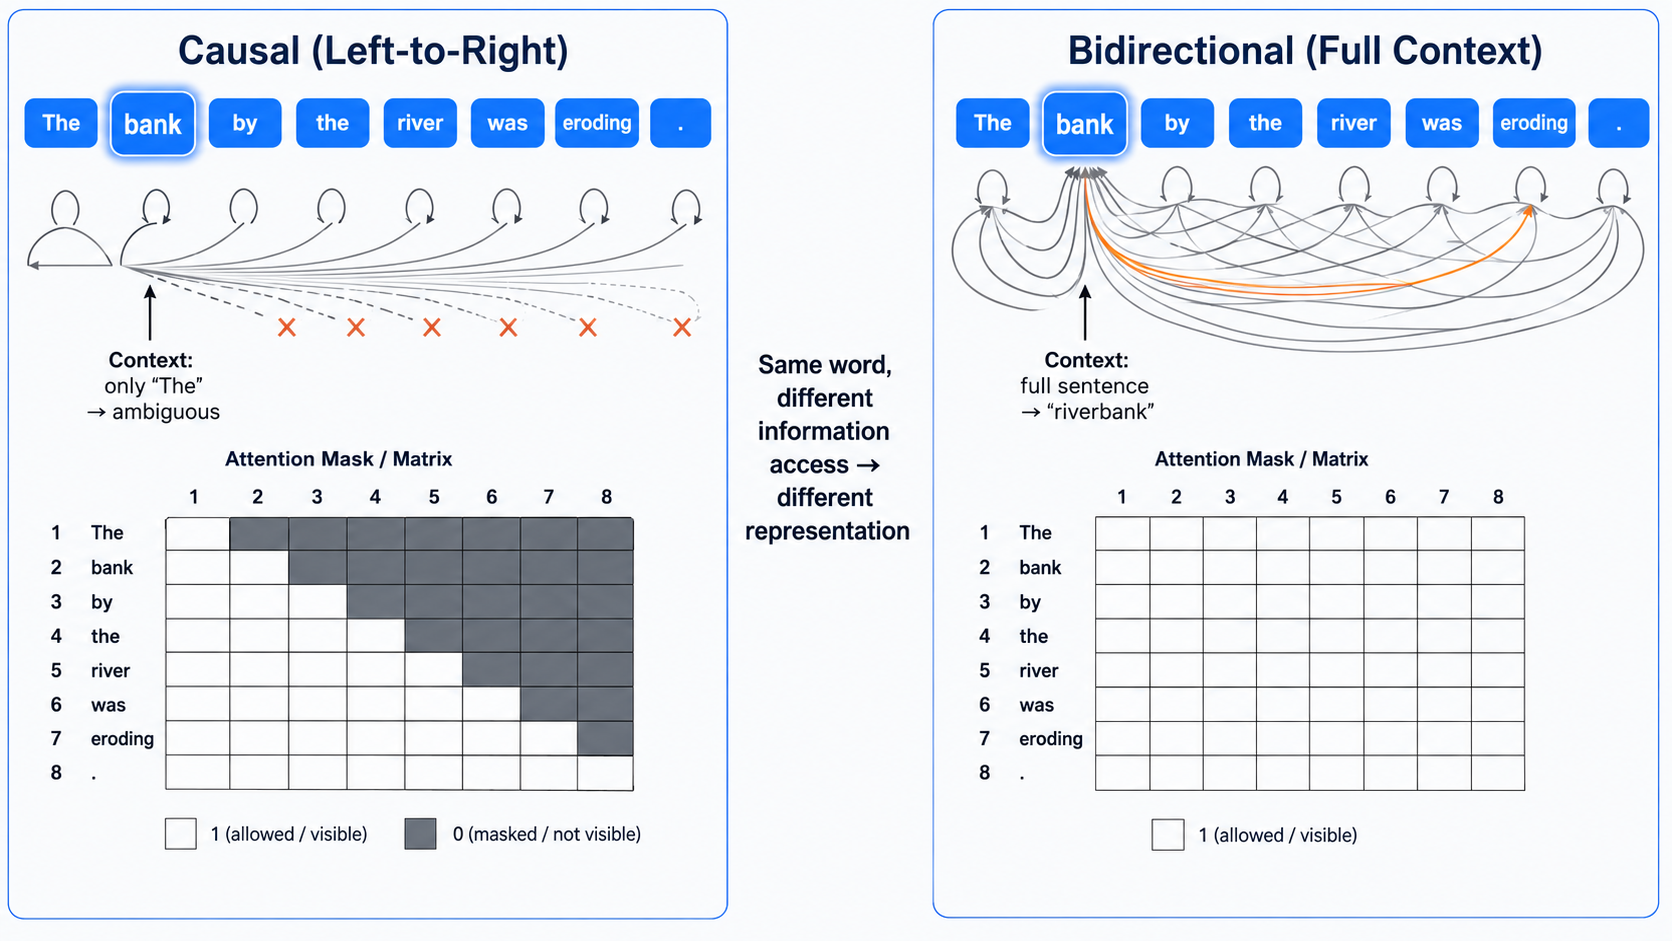
\includegraphics[width=\textwidth]{figures/ch04/causal_vs_bidirectional.png}
\caption{The same sentence processed with causal (left) and bidirectional (right) attention. Bidirectional attention allows ``bank'' to attend to ``river,'' resolving ambiguity instantly.}
\label{fig:causal-vs-bidirectional}
\end{figure}

In that case, the causal mask is actively harmful. Consider the sentence:

\begin{center}
\textit{``The bank by the river was eroding.''}
\end{center}

A left-to-right model processing ``bank'' has only seen ``The''---it cannot know whether ``bank'' means a financial institution or a riverbank. A bidirectional model sees the entire sentence simultaneously. When it processes ``bank,'' it attends to ``river'' and ``eroding'' on the right, disambiguating instantly.

\paragraph{The architectural change is minimal.} Remove the causal mask from the attention computation. That's it. Everything else---multi-head attention, residual stream, layer normalization, FFN blocks---stays identical to Chapter~\ref{ch:decoder-only}. The attention scores become:

\[
  \text{Attention}(\mathbf{Q}, \mathbf{K}, \mathbf{V}) = \text{softmax}\!\left(\frac{\mathbf{Q}\mathbf{K}^\top}{\sqrt{d_k}}\right)\mathbf{V}
\]

No mask applied. Every token attends to every other token. The representation at position $t$ is a function of the \emph{entire} input sequence---past, present, and future.

\paragraph{The consequence is profound.} Bidirectional attention means:
\begin{itemize}[nosep]
  \item Every token's representation is informed by the full context---ideal for understanding tasks.
  \item The model \emph{cannot natively} generate text autoregressively. If every position can see every other position during training, there is no ``next token to predict'' in the causal sense. The model would trivially copy the answer from its own input.
\end{itemize}

This is the fundamental tradeoff of encoder-only models: you gain complete context for representation, but you lose native left-to-right generation.

\begin{quickrecap}
\textbf{Quick Recap.}
\begin{itemize}[nosep,leftmargin=1.5em]
  \item Remove the causal mask $\to$ every token attends to all positions $\to$ bidirectional context.
  \item Bidirectional context makes representations richer (each token ``knows'' its full surroundings).
  \item But it rules out native autoregressive generation.
\end{itemize}
\textit{If we can't train with next-token prediction, what objective do we use?}
\end{quickrecap}

\paragraph{GPT vs.\ BERT at a glance.} The following table summarizes the component-level differences between the two major Transformer branches. The shared components (multi-head attention, FFN, residual stream, layer norm) are identical---the differences are in masking, objective, and interface.

\begin{center}
\begin{tabularx}{\textwidth}{@{}l X X@{}}
\toprule
\textbf{Component} & \textbf{GPT (Ch.~3)} & \textbf{BERT (this chapter)} \\
\midrule
Attention mask & Causal (lower-triangular) & None (full bidirectional) \\
Training objective & Next-token prediction & Masked language modeling (15\%) \\
Prediction targets & Every position ($T-1$ per sequence) & Only masked positions ($\sim$0.15$T$) \\
Input format & Token + position embeddings & Token + position + segment; [CLS], [SEP] \\
Output interface & Generate text (autoregressive) & Produce representations (classify, embed, score) \\
Natural use cases & Chat, writing, code generation & Classification, retrieval, reranking, embeddings \\
Scaling advantage & Signal-dense; generation enables prompting & Bidirectional context; strong per-token representations \\
\bottomrule
\end{tabularx}
\end{center}


%----------------------------------------------------------------------
\section{Masked Language Modeling}
\label{sec:mlm}

BERT's training objective is deceptively simple: hide some tokens, and ask the model to guess what was hidden.

\begin{figure}[ht]
\centering
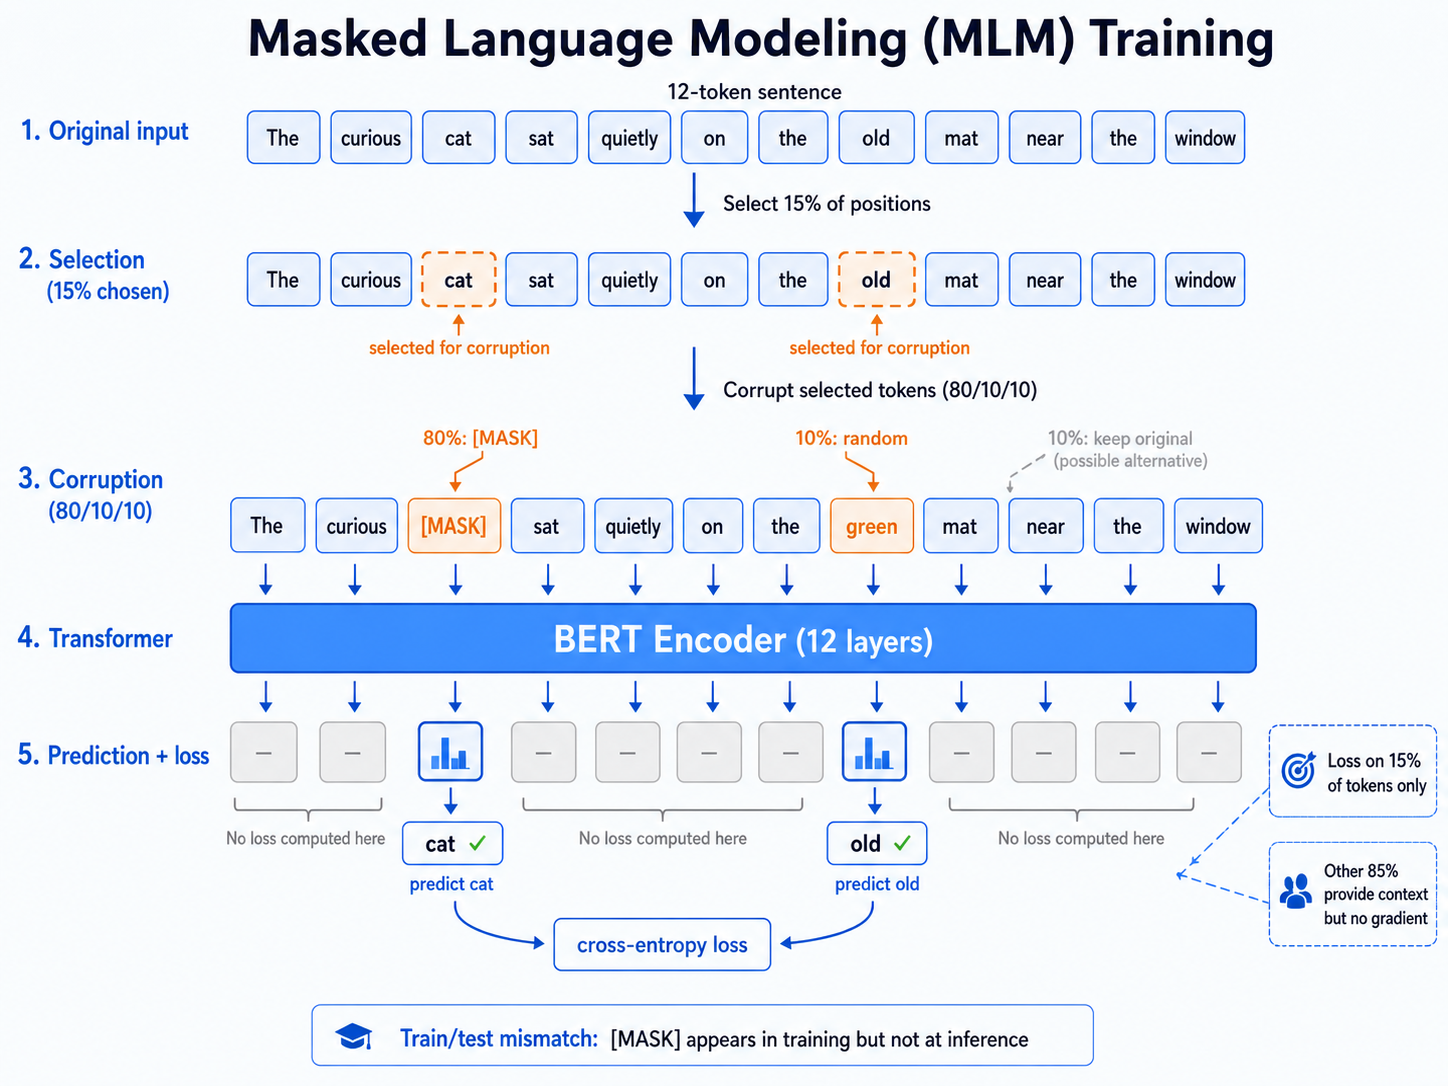
\includegraphics[width=\textwidth]{figures/ch04/mlm_training.png}
\caption{The MLM training procedure: 15\% of tokens are selected, corrupted via the 80/10/10 strategy, and the model predicts the originals only at masked positions.}
\label{fig:mlm-training}
\end{figure}

\paragraph{The procedure.}
\begin{enumerate}[nosep]
  \item Sample a random 15\% of token positions in the input.
  \item For each selected position, apply one of three treatments:
    \begin{itemize}[nosep]
      \item 80\% of the time: replace with \texttt{[MASK]}.
      \item 10\% of the time: replace with a random token from the vocabulary.
      \item 10\% of the time: keep the original token unchanged.
    \end{itemize}
  \item Feed the corrupted input through the Transformer.
  \item Compute cross-entropy loss \emph{only} on the masked positions---the model must predict the original token at each corrupted position.
\end{enumerate}

\paragraph{Why 80/10/10?} The issue is a \textbf{train/test distribution mismatch}. During pretraining, the model sees \texttt{[MASK]} tokens everywhere. During fine-tuning, the input is normal text---no \texttt{[MASK]} tokens at all. If the model were trained with 100\% \texttt{[MASK]} replacement, it would learn to rely heavily on the presence of \texttt{[MASK]} as a signal, and its representations would degrade on normal text.

The 10\% random replacement forces the model to maintain good representations even when the surface token is ``wrong.'' The 10\% unchanged forces it to learn good representations even when the surface token is ``right.'' Together, they make the model robust to the absence of \texttt{[MASK]} at inference time.

\paragraph{Training signal density: the critical comparison.}

\begin{center}
\begin{tabular}{lcc}
\toprule
& \textbf{BERT (MLM)} & \textbf{GPT (next-token)} \\
\midrule
Input: 1000 tokens & & \\
Prediction targets per sequence & 150 (15\%) & 999 (every position) \\
Gradient signal density & 1$\times$ & $\sim$6.7$\times$ \\
\bottomrule
\end{tabular}
\end{center}

\begin{figure}[ht]
\centering
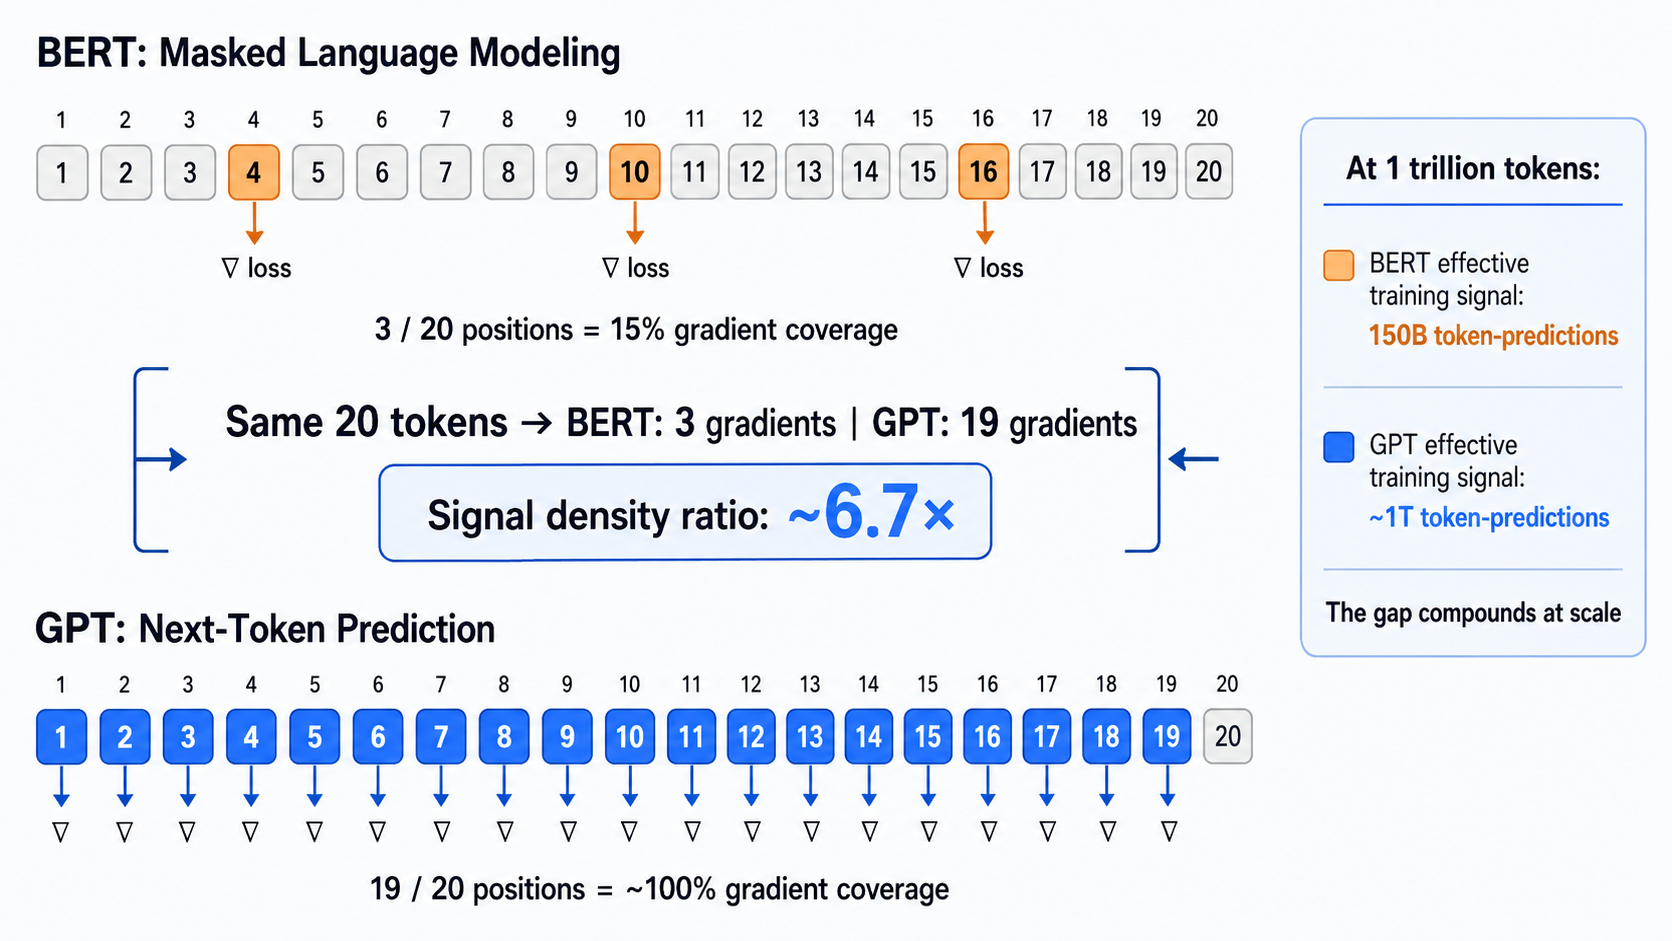
\includegraphics[width=\textwidth]{figures/ch04/signal_density.png}
\caption{Training signal density comparison: BERT computes loss on 15\% of tokens (sparse), while GPT computes loss on every token (dense). Same data, $\sim$6.7$\times$ more gradient signal for GPT.}
\label{fig:signal-density}
\end{figure}

This is not a minor difference. On the same data, with the same compute, GPT extracts nearly 7$\times$ more training signal per batch. At the scale of trillions of tokens, this efficiency gap compounds dramatically. It is one of the central reasons GPT-style models scaled further.

\begin{quickrecap}
\textbf{Quick Recap.}
\begin{itemize}[nosep,leftmargin=1.5em]
  \item MLM: mask 15\% of tokens, predict the originals. Loss computed only on masked positions.
  \item 80/10/10 mitigates the train/test mismatch between pretraining (\texttt{[MASK]} present) and fine-tuning (no \texttt{[MASK]}).
  \item GPT gets $\sim$6.7$\times$ more gradient signal per sequence from the same data. This matters at scale.
\end{itemize}
\textit{We know the objective. What does the input actually look like?}
\end{quickrecap}

\noindent\fbox{\parbox{\dimexpr\textwidth-2\fboxsep-2\fboxrule\relax}{\textbf{Pause and verify.} A 1000-token sequence is fed to BERT. How many tokens are masked? How many prediction targets does BERT get from this sequence? How many does GPT get from the same sequence? Now suppose we used 100\% \texttt{[MASK]} replacement instead of 80/10/10---what problem arises during fine-tuning?}}


%----------------------------------------------------------------------
\section{BERT Input Format: [CLS], [SEP], and Task Heads}
\label{sec:bert-input}

\begin{figure}[ht]
\centering
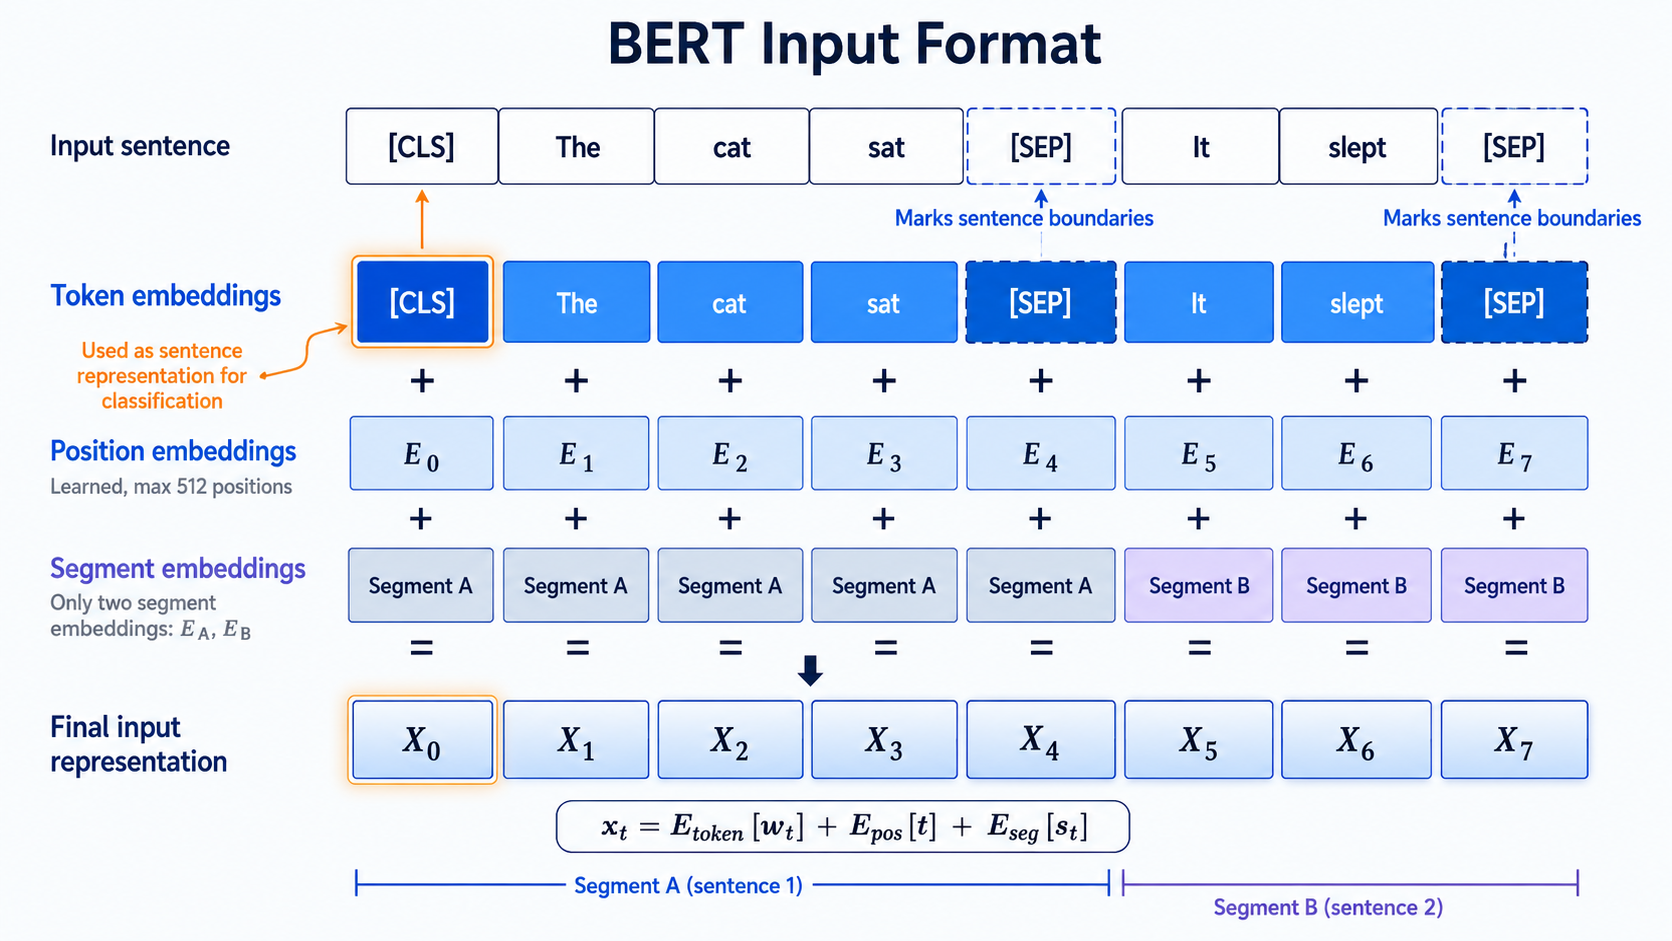
\includegraphics[width=\textwidth]{figures/ch04/bert_input_format.png}
\caption{BERT's input representation: token, position, and segment embeddings are summed. Special tokens \texttt{[CLS]} and \texttt{[SEP]} structure the input for downstream tasks.}
\label{fig:bert-input}
\end{figure}

BERT's input representation has three components summed together:

\[
  \mathbf{x}_t = \mathbf{E}_{\text{token}}[w_t] + \mathbf{E}_{\text{pos}}[t] + \mathbf{E}_{\text{seg}}[s_t]
\]

\paragraph{Token embeddings.} Same as GPT---a learned lookup table $\mathbf{E}_{\text{token}} \in \mathbb{R}^{V \times d_\text{model}}$.

\paragraph{Position embeddings.} Learned absolute position embeddings. Unlike modern GPTs which use RoPE, BERT uses a simple lookup table $\mathbf{E}_{\text{pos}} \in \mathbb{R}^{512 \times d_\text{model}}$. The pretrained table has 512 entries, which is why BERT is typically used with sequences of at most 512 tokens (this is a training choice, not a hard architectural limit).

\paragraph{Segment embeddings.} BERT was designed for \emph{sentence-pair} tasks (e.g., ``Does sentence A entail sentence B?''). The segment embedding $\mathbf{E}_{\text{seg}} \in \mathbb{R}^{2 \times d_\text{model}}$ tells the model which sentence each token belongs to.

\paragraph{Special tokens.}
\begin{itemize}[nosep]
  \item \texttt{[CLS]} is prepended to every input. Its final-layer representation is used as the ``sentence embedding'' for classification tasks.
  \item \texttt{[SEP]} separates the two sentences in a pair.
\end{itemize}

A typical input looks like:

\begin{center}
\texttt{[CLS] The cat sat on the mat [SEP] It was comfortable [SEP]}
\end{center}

\paragraph{Task heads.} After pretraining, BERT's body (the Transformer encoder) produces a $T \times d_\text{model}$ representation matrix. Different tasks attach different heads:

\begin{itemize}[nosep]
  \item \textbf{Classification:} Linear layer on \texttt{[CLS]} representation $\to$ class logits.
  \item \textbf{Token-level tasks} (NER, POS tagging): Linear layer on each token's representation $\to$ per-token labels.
  \item \textbf{Question answering:} Two linear layers predict start and end positions of the answer span.
\end{itemize}

The key insight: the same pretrained body serves all tasks. Only the head changes. This is what made BERT revolutionary---one expensive pretraining run, then cheap fine-tuning for any downstream task.

\begin{quickrecap}
\textbf{Quick Recap.}
\begin{itemize}[nosep,leftmargin=1.5em]
  \item Input = token embedding + position embedding + segment embedding.
  \item \texttt{[CLS]} provides a sentence-level representation; \texttt{[SEP]} marks sentence boundaries.
  \item Task-specific heads are thin linear layers on top of the frozen-then-fine-tuned body.
\end{itemize}
\textit{This ``pretrain one model, fine-tune for many tasks'' idea was genuinely new. How significant was it?}
\end{quickrecap}


%----------------------------------------------------------------------
\section{Pre-train + Fine-tune: The Paradigm BERT Established}
\label{sec:pretrain-finetune}

Before BERT, the dominant approach in NLP was:
\begin{enumerate}[nosep]
  \item Design task-specific architectures for each problem.
  \item Train from scratch on task-specific labeled data.
  \item Optional: initialize word embeddings with Word2Vec/GloVe.
\end{enumerate}

\begin{figure}[ht]
\centering
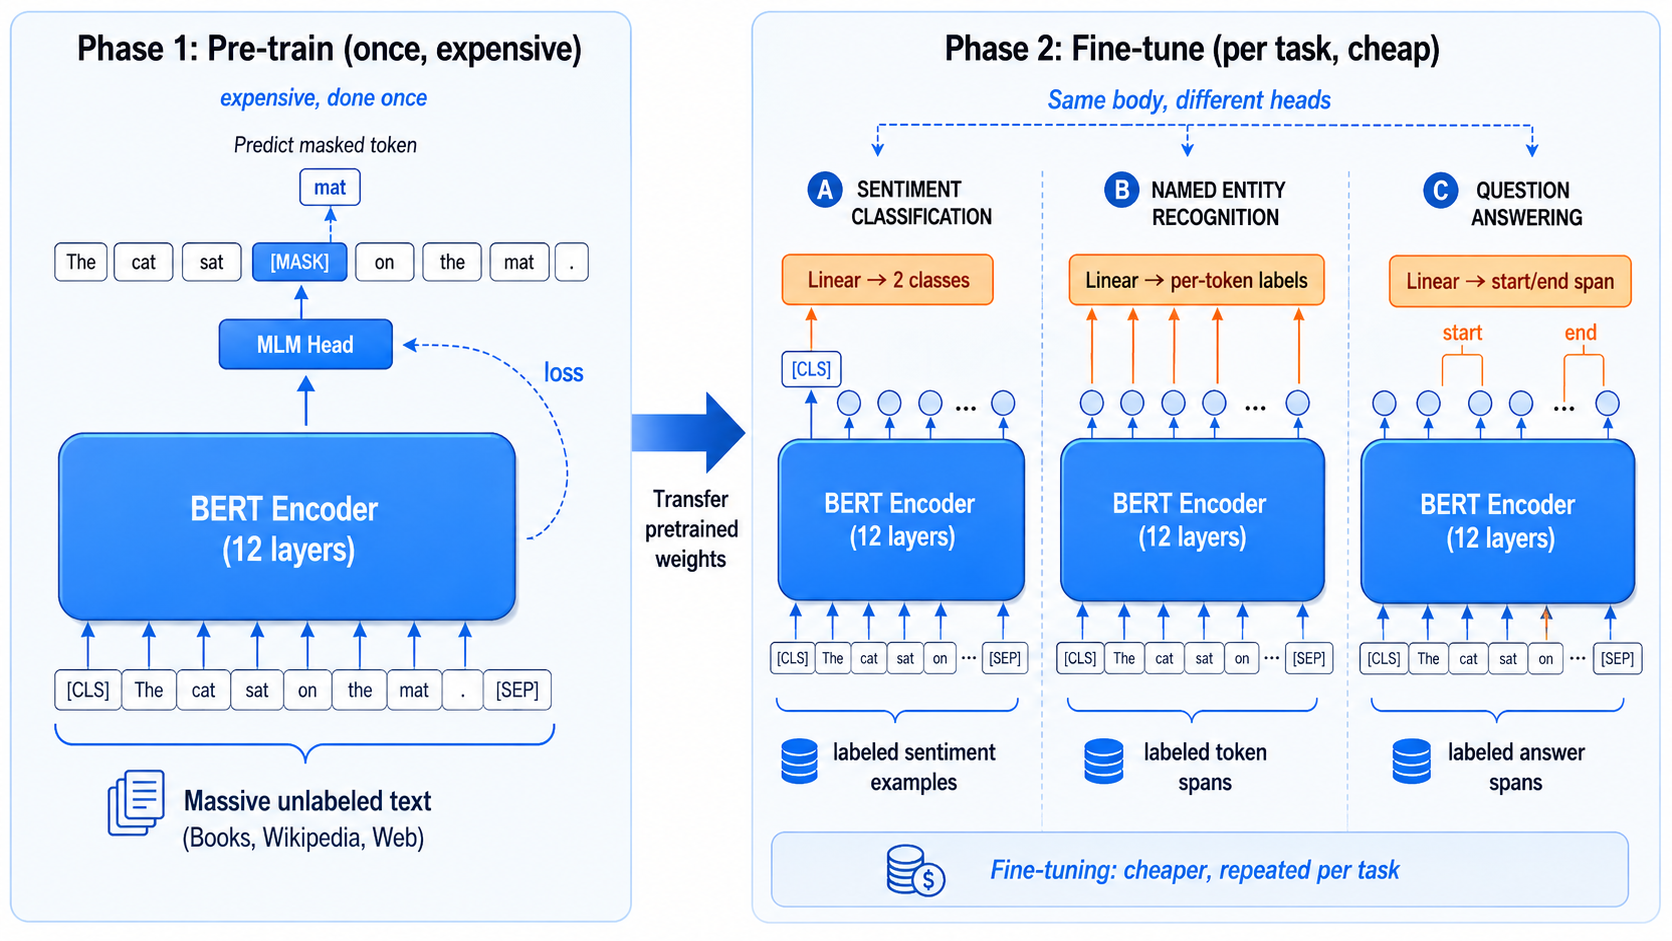
\includegraphics[width=\textwidth]{figures/ch04/pretrain_finetune.png}
\caption{The pre-train + fine-tune paradigm: one pretrained BERT body serves multiple tasks by swapping lightweight task heads. The encoder body (blue) is shared; only the task heads (orange) are new.}
\label{fig:pretrain-finetune}
\end{figure}

BERT introduced a two-stage paradigm:
\begin{enumerate}[nosep]
  \item \textbf{Pre-train:} One large Transformer, trained on massive unlabeled text with MLM. This is expensive but done once.
  \item \textbf{Fine-tune:} Take the pretrained model, add a task-specific head, and fine-tune all parameters on (often small) labeled data. This is cheap and fast.
\end{enumerate}

\paragraph{Why this worked so well:}
\begin{itemize}[nosep]
  \item The pretrained representations encode rich linguistic knowledge---syntax, semantics, world knowledge---learned from billions of words.
  \item Fine-tuning adapts these representations to specific tasks with far less labeled data than training from scratch.
  \item Tasks that previously required large task-specific datasets could often be solved with modest supervised datasets.
\end{itemize}

\paragraph{The historical significance.} Pre-train + fine-tune unified NLP. Before BERT, every task (sentiment, NER, QA, entailment) had its own architecture, its own tricks, its own state of the art. After BERT, one architecture ruled them all---the differences were only in the task head and the fine-tuning data.

This paradigm was so successful that it became the default for many NLU systems from roughly 2019 onward. It was challenged by an even more radical idea: don't fine-tune at all. GPT-3 showed that a sufficiently large model could perform tasks via \emph{in-context learning}---just describe the task in the prompt, and the model adapts without any parameter updates. This was the beginning of the end for BERT's role as the default frontier interface.

\begin{quickrecap}
\textbf{Quick Recap.}
\begin{itemize}[nosep,leftmargin=1.5em]
  \item BERT established: expensive pretraining once $\to$ cheap fine-tuning for each task.
  \item This unified NLP: same architecture, same pretrained weights, different task heads.
  \item GPT-3's in-context learning displaced fine-tuning as the dominant interface---no parameter updates needed.
\end{itemize}
\textit{So if BERT was so successful, why did the field move away from it?}
\end{quickrecap}


%----------------------------------------------------------------------
\section{Why BERT Lost the Frontier Role}
\label{sec:bert-lost}

BERT didn't get worse. The definition of ``good AI'' changed. Three forces converged:

\paragraph{1. BERT cannot natively generate.} By 2022, users expected AI to \emph{write}---emails, code, summaries, stories. BERT can classify, extract, and score, but it is not trained to extend a prompt one token at a time. The user interface of the future was chat, and chat requires generation. This is an \emph{architectural} limitation, not a training issue---no amount of scaling or data can give an encoder-only model native left-to-right generation. BERT was structurally mismatched with the most commercially visible application of AI.

\paragraph{2. Fine-tuning is fragile and expensive.} Each task requires:
\begin{itemize}[nosep]
  \item A labeled dataset.
  \item A training run (even if short).
  \item A separate model copy or adapter for deployment.
\end{itemize}
For 50 tasks, you maintain 50 fine-tuned models. GPT-3 and its successors do all 50 tasks with one model, one deployment, zero fine-tuning---just different prompts. The operational simplicity is overwhelming.

\paragraph{3. Training signal sparsity compounds at scale.} As we saw in \S\ref{sec:mlm}, BERT extracts prediction targets from only 15\% of tokens. GPT uses every token---$\sim$6.7$\times$ more gradient signal per batch. When labs started training on trillions of tokens, this efficiency gap widened. You cannot easily fix this by masking more---empirically, beyond $\sim$15--20\% masking, the remaining context becomes too sparse for accurate prediction. Note: this reason alone would not have displaced BERT (scaling BERT more would still not yield generation), but it made the gap between BERT-scale and GPT-scale investments even less attractive.

\paragraph{The summary verdict:}

\begin{center}
\textit{BERT won the NLU benchmark era but lost the interface war.}
\end{center}

BERT optimized for a world where the output was a label (positive/negative, span start/end, entailment/contradiction). The world decided it wanted the output to be \emph{text}. A model that is not built for generation is a poor fit for chatbots, writing assistants, and coding copilots. BERT was excellent at the benchmark era's tasks, but poorly matched to the next interface.

\begin{quickrecap}
\textbf{Quick Recap.}
\begin{itemize}[nosep,leftmargin=1.5em]
  \item Interface: users want generation. BERT is not a native autoregressive generator---this is architectural, not fixable by scaling.
  \item Operations: fine-tuning per task vs.\ prompting one model. Prompting wins on simplicity.
  \item Signal density: MLM uses 15\% of tokens; next-token prediction uses 100\%. At scale, this compounds the disadvantage.
\end{itemize}
\textit{If BERT lost, why are we still studying it? Because it didn't lose everywhere.}
\end{quickrecap}

\noindent\fbox{\parbox{\dimexpr\textwidth-2\fboxsep-2\fboxrule\relax}{\textbf{Pause and verify.} Name the three forces that displaced BERT from the frontier. For each, is it a structural limitation of encoder-only architectures, or a fixable engineering issue? If a startup asks you to build a chatbot using BERT, what goes wrong---and what would you recommend instead?}}


%----------------------------------------------------------------------
\section{The BERT Family}
\label{sec:bert-family}

BERT spawned a family of encoder-only models that addressed its known weaknesses while preserving its core strength: bidirectional representation learning. The most important descendants:

\begin{center}
\begin{tabularx}{\textwidth}{@{}lX@{}}
\toprule
\textbf{Model} & \textbf{Key improvement over BERT} \\
\midrule
\textbf{RoBERTa} (2019) &
  Remove NSP (next sentence prediction---BERT's secondary objective was too easy and taught shortcuts). Train longer on more data with dynamic masking. Result: stronger representations with no architectural change. \\[6pt]
\textbf{DeBERTa} (2020) &
  Disentangled attention: separate content and position signals rather than adding them into one vector at the input. Better positional reasoning and stronger downstream accuracy. \\[6pt]
\textbf{Sentence-BERT} (2019) &
  Siamese architecture: two BERT encoders share weights, produce sentence embeddings via mean pooling, trained with contrastive loss. Made BERT useful for semantic search and similarity. \\[6pt]
\textbf{BGE / E5 / GTE} (2023--24) &
  Modern encoder-style embedding models. Trained with large-scale contrastive learning on instruction-aware data. Competitive for dense retrieval and semantic similarity. \\
\bottomrule
\end{tabularx}
\end{center}

\begin{figure}[ht]
\centering
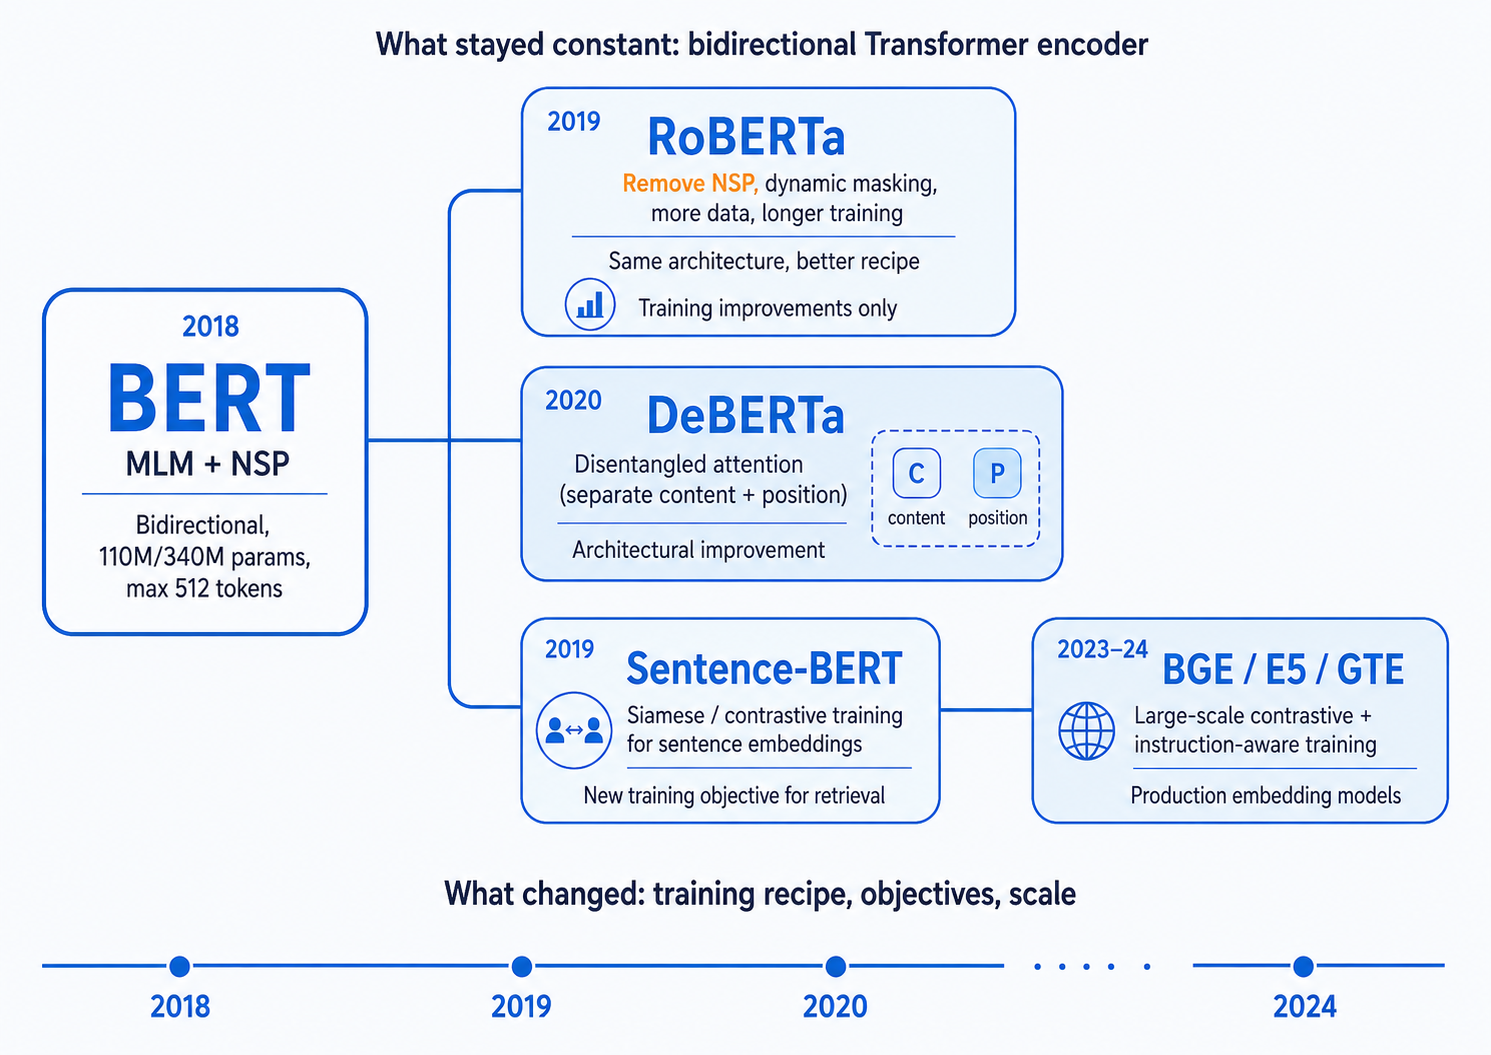
\includegraphics[width=\textwidth]{figures/ch04/bert_family_evolution.png}
\caption{The BERT family tree: each successor addressed a specific limitation while preserving the core bidirectional encoder architecture. Orange highlights the single most impactful lesson: removing NSP.}
\label{fig:bert-family}
\end{figure}

\paragraph{The pattern.} Each successor kept bidirectional attention and representation-learning objectives, but fixed specific failure modes: NSP was harmful (RoBERTa); position handling was rigid (DeBERTa); \texttt{[CLS]} alone was a poor sentence embedding (Sentence-BERT); training data and objectives needed scaling (BGE/E5/GTE).

The BERT lineage is alive and evolving---it just no longer claims to be the universal model. Instead, it has found its niche.


%----------------------------------------------------------------------
\section{BERT Today: Embeddings, Retrieval, and Reranking}
\label{sec:bert-today}

In 2025, BERT-style encoder models are invisible to end users but load-bearing in production systems. Three roles:

\paragraph{1. Dense retrieval (bi-encoder).} Given a query, encode it into a vector. Compare against pre-encoded document vectors via cosine similarity or dot product. Return the nearest neighbors. This is how modern search systems work---billions of documents encoded offline, retrieved in milliseconds.

The encoder model (BGE, E5, GTE, or a fine-tuned BERT) runs once per document at indexing time, and once per query at search time. No generation needed. Bidirectional attention is ideal: the encoder sees the entire document/query and compresses it into a single vector.

\paragraph{2. Cross-encoder reranking.} A bi-encoder is fast but approximate---it compresses each text independently. For higher precision, a \emph{cross-encoder} takes the query and document \emph{together} as input:

\begin{center}
\texttt{[CLS] query text [SEP] document text [SEP]}
\end{center}

The \texttt{[CLS]} representation is passed through a linear layer to produce a relevance score. This is more accurate than bi-encoding because the model can attend across query and document simultaneously. It is also slower---which is why it's used only for reranking the top-$k$ candidates from the retriever.

\paragraph{3. Classification and NLU.} Spam detection, content moderation, intent classification, sentiment analysis---tasks where the output is a label, not text. A compact fine-tuned encoder can run at low latency and low cost, and it often remains the practical choice for high-volume, narrow classification workloads.

\begin{figure}[ht]
\centering
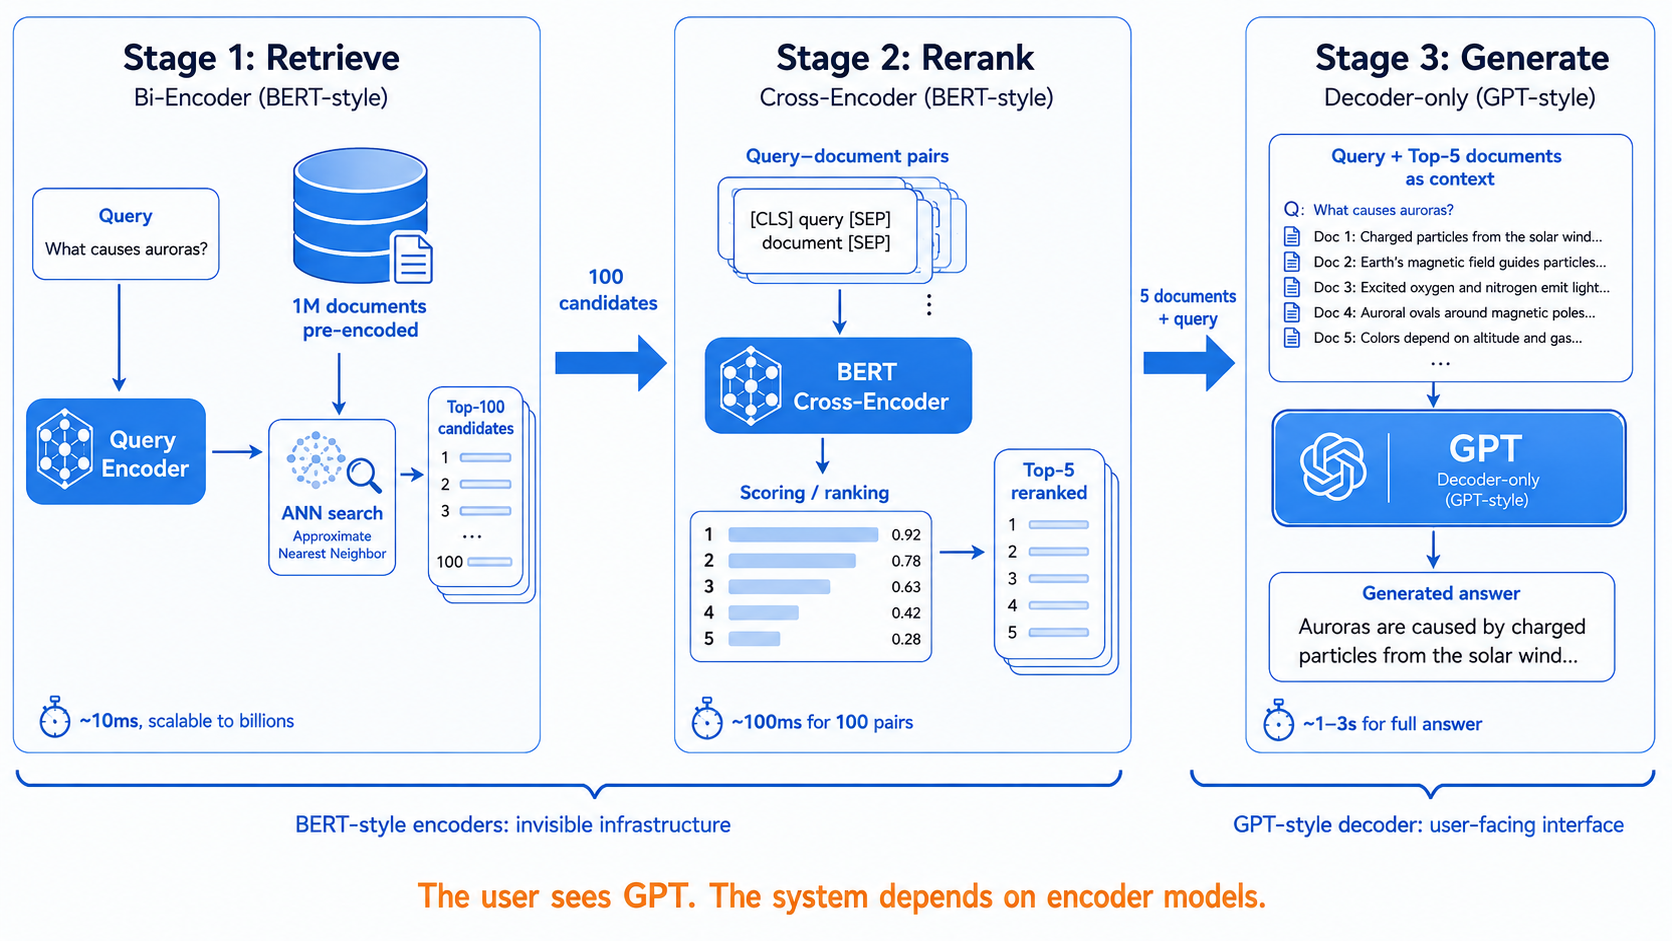
\includegraphics[width=\textwidth]{figures/ch04/rag_pipeline.png}
\caption{A modern RAG pipeline: encoder models (BERT-style) handle retrieval and reranking; a decoder model (GPT-style) generates the final answer. The user sees GPT; the system depends on BERT.}
\label{fig:rag-pipeline}
\end{figure}

\paragraph{The modern RAG pipeline.} Here is where BERT and GPT coexist:

\begin{enumerate}[nosep]
  \item \textbf{Retriever} (encoder model): query $\to$ vector $\to$ ANN search $\to$ top-100 candidates.
  \item \textbf{Reranker} (cross-encoder): score each (query, candidate) pair $\to$ top-5.
  \item \textbf{Generator} (GPT-style LLM): synthesize an answer using the top-5 as context.
\end{enumerate}

\textit{The user may see GPT. The system often depends on encoder models.}

\begin{quickrecap}
\textbf{Quick Recap.}
\begin{itemize}[nosep,leftmargin=1.5em]
  \item BERT-style models power retrieval (bi-encoder), reranking (cross-encoder), and classification.
  \item These are infrastructure roles: invisible to users, load-bearing for systems.
  \item In RAG pipelines, encoder models retrieve and rerank; GPT generates.
\end{itemize}
\textit{Is this the end of the story? Or could representation learning return to the frontier?}
\end{quickrecap}


%----------------------------------------------------------------------
\section{Beyond BERT: JEPA and Latent-Space Prediction}
\label{sec:jepa}

BERT proved that ``mask some input, predict what's missing'' is a powerful self-supervised objective. But it has a fundamental limitation: it predicts in \textbf{input space}. The model must reconstruct the exact token that was masked---which means it spends capacity distinguishing between synonyms, resolving surface-level ambiguity, and modeling low-level statistics of text.

What if we keep the masking intuition but predict in a more abstract space?

\begin{figure}[ht]
\centering
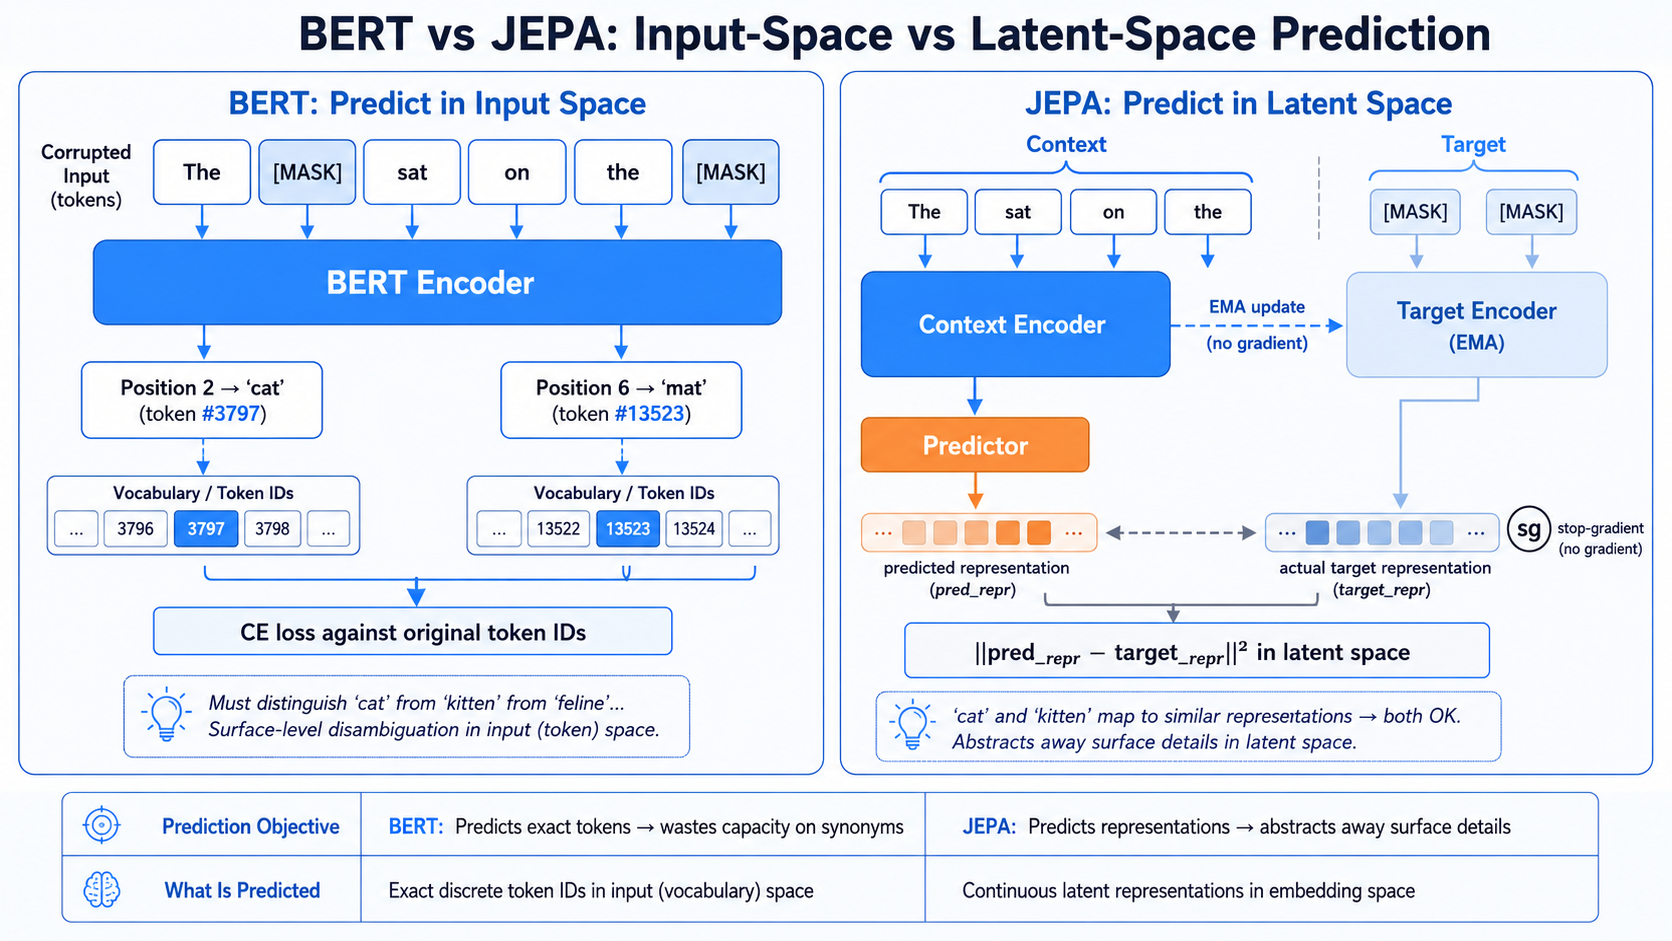
\includegraphics[width=\textwidth]{figures/ch04/bert_vs_jepa.png}
\caption{BERT predicts masked tokens in input space (left); JEPA predicts masked representations in latent space (right). Both learn through masking, but JEPA avoids surface-level reconstruction.}
\label{fig:bert-vs-jepa}
\end{figure}

\paragraph{The JEPA architecture.} JEPA (Joint-Embedding Predictive Architecture) consists of three components:

\begin{enumerate}[nosep]
  \item \textbf{Context encoder}: processes the unmasked portion of the input $\to$ context representation.
  \item \textbf{Target encoder}: processes the masked portion $\to$ target representation. Updated via exponential moving average (EMA) of the context encoder---not by gradient descent directly.
  \item \textbf{Predictor}: a lightweight network that takes the context representation and predicts the target representation.
\end{enumerate}

The loss is computed in \emph{representation space}:
\[
  \mathcal{L} = \| \text{Predictor}(z_\text{context}) - \text{sg}(z_\text{target}) \|^2
\]
where $\text{sg}$ denotes stop-gradient (the target encoder is not updated by this loss directly). In practice, the predictor also receives positional information about \emph{which} regions are masked, so it knows what to predict---this is omitted above for clarity.

\paragraph{Why predict in latent space?}

\begin{center}
\begin{tabularx}{\textwidth}{@{}lXX@{}}
\toprule
& \textbf{BERT} & \textbf{JEPA} \\
\midrule
Predicts & Masked token IDs & Latent representations \\
Space & Input (discrete, surface) & Latent (continuous, abstract) \\
Reconstruction burden & Synonyms, surface statistics & Reduced---abstracts away some details \\
Multimodal? & Awkward (different decoders) & Natural (same latent space) \\
\bottomrule
\end{tabularx}
\end{center}

BERT's cross-entropy loss is sensitive to surface form: if the masked position held ``happy'' but the model assigns high probability to ``glad'' or ``pleased''---semantically equivalent---it is still penalized. The loss pushes the model to model surface-level token distributions, not just deeper semantics. JEPA reduces this pressure: its loss operates in representation space, so semantically similar content can map to nearby representations without committing to a specific discrete token.

\paragraph{Preventing collapse.} If JEPA just minimizes the distance between predicted and target representations, the trivial solution is: make all representations identical (collapse to a constant). Practical JEPA systems avoid this through stop-gradient targets, an EMA-updated target encoder, masking design, and predictor asymmetry. The target changes slowly while the context encoder trains, making collapse less attractive than learning informative representations.

\paragraph{Why JEPA is considered a potential challenger to GPT.}

The argument, most forcefully made by Yann LeCun, has several layers:

\begin{enumerate}[nosep]
  \item \textbf{Autoregressive generation operates token-by-token in discrete space.} This is fundamentally ill-suited for modeling continuous phenomena (physics, video, spatial reasoning). JEPA operates in continuous latent space.
  \item \textbf{Next-token prediction learns surface statistics, not world models.} A model that can predict the next word does not necessarily understand the causal structure of the world. JEPA's objective---predict abstract future states---is closer to what a ``world model'' requires.
  \item \textbf{Planning in latent space.} If a model can predict future representations, it can evaluate the consequences of actions without generating full sequences. This enables hierarchical planning---something current LLMs struggle with.
\end{enumerate}

\paragraph{Current status and honest assessment.}

I-JEPA (images, 2023), V-JEPA (video, 2024), and V-JEPA~2 (2025) have demonstrated that JEPA learns strong visual representations without pixel-level reconstruction. V-JEPA~2 has been positioned by Meta as a video-based world model for visual understanding, prediction, planning, and robot control~\cite{vjepa2meta2025}.

However, JEPA's text-domain success remains limited. Natural language is already discrete (tokens), which reduces JEPA's ``no reconstruction in continuous space'' advantage. The most capable text models in 2025 are still decoder-only autoregressive Transformers. Whether JEPA or JEPA-inspired architectures will eventually challenge GPT-style models for language tasks is an open question---but the theoretical arguments are serious enough that the research community is actively pursuing this direction.

\begin{quickrecap}
\textbf{Quick Recap.}
\begin{itemize}[nosep,leftmargin=1.5em]
  \item BERT predicts masked tokens in input space. JEPA predicts masked representations in latent space.
  \item Latent-space prediction avoids wasting capacity on surface statistics and naturally supports multimodal learning.
  \item JEPA is validated in vision/video but not yet dominant in text. The theoretical case is serious; the empirical story is still unfolding.
\end{itemize}
\end{quickrecap}

\paragraph{The architecture--objective design space.} With GPT, BERT, and JEPA, you have now seen three points in a larger design space. The lesson is general: \emph{capability emerges from the coupling of architecture, masking strategy, and training objective---not from any one component alone.}

\begin{center}
\begin{tabularx}{\textwidth}{@{}l l l X@{}}
\toprule
\textbf{System} & \textbf{Attention} & \textbf{Objective} & \textbf{Emergent capability} \\
\midrule
GPT & Causal & Next-token prediction & Fluent generation; in-context learning at scale \\
BERT & Bidirectional & Masked token prediction & Rich per-token representations; classification and retrieval \\
JEPA & Non-causal / masked & Latent-space prediction & Abstract world modeling; planning without reconstruction \\
\bottomrule
\end{tabularx}
\end{center}

The Transformer block itself is a general-purpose compute primitive. What you \emph{do} with it---which positions can attend to which, and what the model is asked to predict---determines what kind of intelligence emerges. This is perhaps the deepest lesson of Part~I: the same mechanism, under different constraints, produces fundamentally different machines.


%----------------------------------------------------------------------
\section{Failure Modes and Misconceptions}
\label{sec:bert-failures}

Before summarizing, let us confront five misconceptions that commonly arise after reading about BERT and encoder-only models. Each can cause confusion in later chapters on retrieval, fine-tuning, and system design.

\begin{itemize}
  \item \textbf{``\texttt{[CLS]} is a good sentence embedding out of the box.''} It is not. Without fine-tuning or contrastive training, the \texttt{[CLS]} vector from a pretrained BERT is a poor sentence representation---often worse than simple mean pooling of all token embeddings. Sentence-BERT and modern embedding models exist precisely to fix this.

  \item \textbf{``BERT understands language; GPT just predicts.''} This is a false dichotomy. Both models learn statistical patterns from text. ``Understanding'' is an overloaded term. BERT's bidirectional context gives it better per-token representations for classification-style tasks; GPT's autoregressive training gives it the ability to generate coherent continuations. Neither ``understands'' in the human sense.

  \item \textbf{``Fine-tuning always helps.''} On very small datasets ($<$100 examples), fine-tuning can overfit catastrophically---the model memorizes the training set and loses its pretrained generalization. In such cases, few-shot prompting with a GPT-style model or careful regularization (learning rate warmup, early stopping, frozen lower layers) is often more robust.

  \item \textbf{``BERT is obsolete.''} BERT-base is a 2018 model. Its architecture is indeed outdated. But the \emph{encoder-only paradigm} is alive---BGE, E5, GTE, and other modern embedding models are architecturally similar (bidirectional Transformer, contrastive training) and are state-of-the-art for retrieval tasks in 2025.

  \item \textbf{``JEPA will replace transformers.''} JEPA is a \emph{training framework}, not an architecture. I-JEPA and V-JEPA use Vision Transformers as their encoder. JEPA and Transformers are not competitors---JEPA defines what to predict; the Transformer defines how to compute representations.
\end{itemize}


%----------------------------------------------------------------------
\section{Trick Table}

\noindent
\begin{tabularx}{\textwidth}{@{}>{\raggedright\arraybackslash}p{2.8cm}
                              >{\raggedright\arraybackslash}p{2.8cm}
                              >{\raggedright\arraybackslash}p{3.2cm}
                              X@{}}
\toprule
\textbf{Trick} & \textbf{When to use} & \textbf{Expected effect} & \textbf{Failure signal} \\
\midrule
Dynamic masking &
  Always (RoBERTa-style) &
  Different masks each epoch; prevents memorization of mask patterns &
  Static masking may lead to slight overfitting on frequent mask positions \\[4pt]
Remove NSP &
  Default for modern encoder pretraining &
  Removes a too-easy secondary objective that teaches shortcuts &
  NSP can teach shortcuts and contribute little useful signal \\[4pt]
Mean pooling over \texttt{[CLS]} &
  When using BERT for sentence embeddings without fine-tuning &
  More stable sentence representation from pretrained model &
  \texttt{[CLS]} without fine-tuning is unreliable \\[4pt]
Cross-encoder for reranking &
  When bi-encoder recall is good but precision is insufficient &
  Joint query-document attention; much higher relevance accuracy &
  Too slow for first-stage retrieval over millions of documents \\[4pt]
Contrastive fine-tuning &
  Building embedding/retrieval models &
  Aligns similar texts in embedding space; state-of-the-art for retrieval &
  Requires careful hard-negative mining; poor negatives $\to$ weak model \\
\bottomrule
\end{tabularx}


\begin{takeaways}
\begin{itemize}[leftmargin=1.2em, itemsep=4pt]
  \item Encoder-only Transformers remove the causal mask, enabling bidirectional attention. This produces richer per-token representations but rules out native autoregressive generation.
  \item \textbf{Masked Language Modeling} trains the model to predict 15\% of tokens from bidirectional context. The 80/10/10 strategy mitigates the train/test distribution mismatch.
  \item BERT established the \textbf{pre-train + fine-tune} paradigm: one expensive pretraining run, then cheap task-specific fine-tuning. This unified many NLU workflows.
  \item BERT lost the frontier role because: (1) it is not a native generator, (2) per-task fine-tuning is operationally expensive compared to prompting, and (3) MLM's signal density is $\sim$6.7$\times$ lower than next-token prediction at scale.
  \item BERT-style models remain dominant for \textbf{embeddings, retrieval, reranking, and classification}---tasks where the output is a vector or a label, not generated text.
  \item \textbf{JEPA} preserves BERT's ``mask and predict'' spirit but moves prediction to latent space. This avoids reconstruction waste, supports multimodal learning, and opens the door to latent-space planning.
  \item GPT won the user interface. BERT remains the infrastructure. JEPA asks whether future AI needs representation-first architectures more than generation-first ones.
\end{itemize}
\end{takeaways}


\section*{Lab 4: Same Block, Different Capability}

\subsection*{Goal}

Lab~2 removed ingredients from a working model. Lab~3 built one up from scratch. Lab~4 uses a third method: \textbf{controlled comparison}. You take two pretrained models---DistilBERT (bidirectional, \textasciitilde66M params) and DistilGPT2 (causal, \textasciitilde82M params)---and measure exactly where each one excels, using the same data, the same probe, and the same evaluation. The central finding: bidirectional representations are measurably better for understanding tasks, while causal representations are better for generation.

\subsection*{Expected Time}

Core (Experiments~0--3): 3--4 hours. This lab is lighter on compute than Lab~3 because you use pretrained models, not training from scratch.

\subsection*{Setup}

See \texttt{labs/ch04/README.md} for the full specification. You will need the \texttt{transformers} and \texttt{datasets} libraries. Models are loaded from HuggingFace. The primary dataset is SST-2 (sentiment classification, positive/negative movie reviews).

\noindent This is a \textbf{diagnosis-first lab}: your time goes into probing pretrained representations, interpreting accuracy gaps, and comparing model interfaces---not building or training models from scratch.

\subsection*{Experiment 0: Polysemy Sanity Check}

\textbf{Corresponds to:} \S4.2 (bidirectional attention). Closes the loop from Lab~1 Exp~0.

\textbf{Goal:} Show that BERT's contextual embeddings distinguish word senses that static embeddings cannot.

\begin{enumerate}[nosep]
    \item Pick polysemous words: ``bank'' (financial/river), ``bat'' (sports/animal), ``light'' (illumination/weight).
    \item For each word in each sense-context, extract: (a) the raw token embedding (static, no context), and (b) the last-layer hidden state (contextual).
    \item Compute cosine similarity between senses. Static embeddings should be nearly identical ($\approx 1.0$) regardless of sense. Contextual embeddings should show clearly lower similarity across senses.
\end{enumerate}

\textbf{Report:} Cosine similarity table, plus one paragraph connecting to Lab~1's static embedding limitation.

\subsection*{Experiment 1: Frozen Probe on SST-2 (Centerpiece)}

\textbf{Corresponds to:} \S4.2, \S4.6.

\textbf{Goal:} Measure how much task-relevant information different encoder types capture in their pretrained representations.

Freeze three encoders and train only a single linear classifier on SST-2 (5000 train / 872 val):

\begin{enumerate}[nosep]
    \item \textbf{Static embeddings.} Mean of token embeddings from the embedding layer (no Transformer processing).
    \item \textbf{DistilGPT2.} Last non-pad token's hidden state (the natural pooling for causal models).
    \item \textbf{DistilBERT.} \texttt{[CLS]} token's hidden state (the natural pooling for BERT).
\end{enumerate}

\textbf{Key deliverable:} One bar chart showing validation accuracy for all three. This is the centerpiece figure of Lab~4---it should make the value of bidirectional context immediately visible.

\textbf{What to look for:} Static $<$ GPT $<$ BERT. The gap between GPT and BERT quantifies the value of seeing right-context. If GPT is close to BERT, consider why: the last token in a full sentence has already seen the entire input via causal attention.

\subsection*{Experiment 2: Fine-tune Comparison}

\textbf{Corresponds to:} \S4.5 (pre-train + fine-tune).

\textbf{Goal:} Check whether full fine-tuning closes the gap observed in Experiment~1.

\begin{enumerate}[nosep]
    \item Fine-tune DistilBERT end-to-end on SST-2 (3 epochs, lr=$2 \times 10^{-5}$).
    \item Fine-tune DistilGPT2 end-to-end with the same hyperparameters.
    \item Compare validation accuracy.
\end{enumerate}

\textbf{What to look for:} The gap should shrink compared to frozen probing. GPT \emph{can} do classification---it is not architecturally incapable. But if BERT still leads, the advantage is structural, not just a training artifact. The insight: frozen probing measures \emph{what the representation already knows}; fine-tuning measures \emph{what it can learn to do}. The difference is the adaptation cost of overcoming interface mismatch.

\subsection*{Experiment 3: Generation Flip}

\textbf{Corresponds to:} \S4.6 (why BERT lost the frontier role).

\textbf{Goal:} Show the other side of the capability tradeoff. GPT generates fluently; BERT cannot.

\begin{enumerate}[nosep]
    \item Give DistilGPT2 prompts like ``The movie was absolutely'' and generate 50 tokens. Observe: coherent continuation.
    \item Give DistilBERT sentences with \texttt{[MASK]} tokens and predict fillers. Observe: single-token prediction only.
    \item Attempt ``generation'' with BERT via iterative mask filling. Observe: awkward, incoherent, fundamentally not what the model was built for.
\end{enumerate}

\textbf{Report:} Side-by-side outputs. One paragraph explaining the architectural reason: bidirectional attention means every position sees every other position, making left-to-right autoregressive generation impossible without external scaffolding.

\subsection*{Report Question}

\begin{quote}
Chapter~4 claims that BERT won representations while GPT won generation. Does your Lab~4 data support this claim? Specifically: (a) what is the frozen-probe accuracy gap, and what does it tell you about pretrained representation bias? (b) does fine-tuning close this gap completely? (c) can BERT generate coherent text? What architectural property prevents it?
\end{quote}


\section{Summary}

\paragraph{What this chapter built.} Chapter~\ref{ch:decoder-only} assembled a generator---a machine that extends prefixes. This chapter assembled its complement: a \emph{representer}---a machine that reads a complete input and produces a rich, contextual embedding for each token. The architectural difference is one line of code (remove the causal mask), but the consequences are far-reaching: different training objective, different capabilities, different role in the AI ecosystem.

\paragraph{The rise and fall.} BERT's pre-train + fine-tune paradigm unified NLP and dominated benchmarks for years. It lost the frontier not because its representations got worse, but because the world decided it wanted AI that \emph{talks back}. Chat requires native generation; BERT is not built for that interface. The simplicity of prompting one large autoregressive model displaced the complexity of maintaining fine-tuned specialists.

\paragraph{Where BERT lives now.} Behind every RAG system, every semantic search engine, every content moderator---encoder-only models encode, retrieve, rerank, and classify. They are the infrastructure layer: invisible to users, essential to systems. GPT is the face; BERT is the backbone.

\paragraph{The frontier question.} JEPA suggests that masked prediction need not happen in input space. By predicting in latent space, we avoid surface-level reconstruction and enable world modeling. If this direction succeeds, BERT's core insight---learn representations by predicting masked content---will return to the frontier in a more powerful form. The story is not over.

\medskip
\noindent\textit{Self-check: Can you explain why removing the causal mask prevents generation? Can you compute the signal density gap between MLM and next-token prediction? Can you describe BERT's role in a RAG pipeline? Can you articulate the difference between BERT's input-space prediction and JEPA's latent-space prediction? If any point is unclear, re-read the corresponding section.}

\medskip
\noindent\textbf{What's next.}\quad We have now covered both major Transformer branches: decoder-only (Chapter~\ref{ch:decoder-only}) for generation and encoder-only (this chapter) for representation. The next chapter turns to how these models are actually trained: optimization, learning rate schedules, distributed training, and the engineering required to make pretraining work at scale.


\section*{Key Equations at a Glance}

\begin{center}
\renewcommand{\arraystretch}{1.6}
\begin{tabularx}{\textwidth}{@{}lX@{}}
\toprule
Component & Equation \\
\midrule
Bidirectional attention & $\text{Attn}(\mathbf{Q}, \mathbf{K}, \mathbf{V}) = \text{softmax}\!\left(\frac{\mathbf{Q}\mathbf{K}^\top}{\sqrt{d_k}}\right)\mathbf{V}$ \quad (no causal mask) \\[4pt]
BERT input & $\mathbf{x}_t = \mathbf{E}_\text{token}[w_t] + \mathbf{E}_\text{pos}[t] + \mathbf{E}_\text{seg}[s_t]$ \\[4pt]
MLM loss & $\mathcal{L}_\text{MLM} = -\frac{1}{|\mathcal{M}|}\sum_{t \in \mathcal{M}} \log P_\theta(w_t \mid \mathbf{x}_{\backslash \mathcal{M}})$ \\[4pt]
Signal density & BERT: $0.15T$ targets/seq \quad vs.\quad GPT: $(T-1)$ targets/seq \\[4pt]
JEPA loss & $\mathcal{L}_\text{JEPA} = \| \text{Predictor}(z_\text{context}) - \text{sg}(z_\text{target}) \|^2$ \\
\bottomrule
\end{tabularx}
\end{center}


\section*{Key Readings}

\begin{enumerate}
  \item \textbf{Devlin et al., ``BERT: Pre-training of Deep Bidirectional Transformers for Language Understanding'' (2019)}~\cite{devlin2019bert}. The original paper. Focus on: the MLM objective design, the 80/10/10 strategy rationale, and the fine-tuning recipe. Note how simple the architecture is compared to the engineering surrounding it.

  \item \textbf{Liu et al., ``RoBERTa: A Robustly Optimized BERT Pretraining Approach'' (2019)}~\cite{liu2019roberta}. The definitive ablation study on BERT's design choices. Shows that NSP hurts, dynamic masking helps, and longer training on more data matters more than architectural changes.

  \item \textbf{Reimers \& Gurevych, ``Sentence-BERT: Sentence Embeddings using Siamese BERT-Networks'' (2019)}~\cite{reimers2019sentence}. How to turn BERT from a classification model into an embedding model. The foundation of modern semantic search.

  \item \textbf{Assran et al., ``Self-Supervised Learning from Images with a Joint-Embedding Predictive Architecture'' (I-JEPA, 2023)}~\cite{assran2023ijepa}. The first empirical validation of JEPA. Focus on: why predicting in latent space outperforms pixel-level reconstruction for learning semantic features.

  \item \textbf{Bardes et al., ``V-JEPA'' (2024)}~\cite{bardes2024vjepa}. Extension to video. Demonstrates that JEPA can learn temporal dynamics without explicit reconstruction---a key step toward world models.
\end{enumerate}
